
%%%%%%%%%%%%%%%%%%%%%%%%%%%%%%%%%%%%%%%%%%%%%%%%%%%%%%%%%%%%%%%%%%%%%%%%%%%%%%%%
%2345678901234567890123456789012345678901234567890123456789012345678901234567890
%        1         2         3         4         5         6         7         8

\documentclass[preprint,12pt]{elsarticle}  % Comment this line out if you need a4paper

\usepackage[utf8]{inputenc}
\usepackage{amsmath, mleftright}
\usepackage{bm}
\usepackage{amssymb}
\usepackage{graphicx}
\usepackage{booktabs}
\usepackage{mathrsfs}
\usepackage{amsbsy}
% \usepackage{caption}
\usepackage[center]{caption}
\usepackage{float}
\usepackage{subcaption}
\usepackage{varwidth}
\usepackage{algorithm}
\usepackage{yhmath}
\usepackage{tabularx}
\usepackage{rotating}
\usepackage[table]{xcolor}
\definecolor{grey}{rgb}{0.9,0.9,0.9}
\usepackage[noend]{algpseudocode}
\usepackage{dsfont}
\usepackage{environ}
\usepackage[framemethod=TikZ]{mdframed}
\usepackage{multirow}
\usepackage{algorithm}
\usepackage{accents}\newcommand\addtag{\refstepcounter{equation}\tag{\theequation}}
\usepackage{etoolbox}
\usepackage{graphicx}
\usepackage{siunitx}
\usepackage{rotating}
\usepackage{enumerate}
\usepackage{hyperref}
\usepackage{relsize}
\usepackage{gensymb}
\usepackage{color}
\usepackage{comment}
\usepackage{xparse}
\usepackage{mathtools}
\usepackage[T1]{fontenc}
\newcommand{\comFB}[1]{~\linebreak\noindent\colorbox{yellow}{\parbox{\dimexpr\columnwidth-1\fboxsep}{[FB: #1]}}}
\newcommand{\comEC}[1]{~\linebreak\noindent\colorbox{green}{\parbox{\dimexpr\columnwidth-1\fboxsep}{[EC: #1]}}}
\newcommand{\comTEMPO}[1]{~\linebreak\noindent\colorbox{gray}{\parbox{\dimexpr\columnwidth-1\fboxsep}{[#1]}}}
%%% Customized commands
%%% example
\newcommand\myNewCommand{\mathbf{\texttt{my new command}}}

\newcommand{\mvec}[1]{\bm{#1}}
\newcommand{\dmvec}[1]{\dot{\mvec{{#1}}}}
\newcommand{\ddmvec}[1]{\ddot{\mvec{{#1}}}}

\newcommand{\st}{\text{s.t.}}
\newcommand{\g}{\mvec{g}}
\newcommand{\q}{\mvec{q}}
\newcommand{\dq}{\dmvec{q}}
\newcommand{\ddq}{\ddmvec{q}} 


\title{\LARGE \bf
Optimal Propulsion Techniques to Generate Non-Twisting Somersaults on Trampoline.
}
\author{Eve Charbonneau\textsuperscript{a,*}, François Bailly\textsuperscript{a} and Mickaël Begon\textsuperscript{a}% <-this % stops a space
\thanks{\textsuperscript{a}\,Laboratoire de Simulation et Modélisation du Mouvement, Faculté de Médecine, Université de Montréal, Laval, QC, Canada}%
\thanks{\textsuperscript{*}\,eve.charbonneau.1@umontreal.ca}
}

%%% User commands

\usepackage{pdfrender}
\DeclareRobustCommand*{\pmbb}[1]{%
  \textpdfrender{
    TextRenderingMode=Stroke,
    LineWidth=.1pt,
  }{#1}%
}
\NewEnviron{comeq}{%
\par\vspace{0ex}
\begin{mdframed}[outerlinewidth=0.5,leftmargin=10,rightmargin=-10pt,backgroundcolor=white,hidealllines=true,leftline=true,
innertopmargin=0pt,splittopskip=0, skipbelow=\baselineskip, innerbottommargin=0pt%
skipabove=0ex]%
\vspace{-0ex}\hspace{0pt}\textit{Proof:}%
\itshape
\begin{equation*} 
\begin{split}
\BODY
\end{split}
\end{equation*}
\end{mdframed}
}
\newcommand{\pd}[2]{\frac{\partial #1}{\partial #2}}
\def\abs{\operatorname{abs}}
\def\argmax{\operatornamewithlimits{arg\,max}}
\def\argmin{\operatornamewithlimits{arg\,min}}
\def\diag{\operatorname{Diag}}
\newcommand{\eqRef}[1]{(\ref{#1})}
\newcommand{\dbtilde}[1]{\accentset{\approx}{#1}}
\hypersetup{
    colorlinks=true,
    linkcolor=blue,
    filecolor=magenta,      
    urlcolor=blue,
}
\hyphenpenalty=100000

\begin{document}


\thispagestyle{empty}
\pagestyle{empty}

\begin{abstract}
% Aerial twisting techniques have gained coaches' interest since the flight time is part of the score in trampoline. 
% As these techniques are not intuitive, computer simulation has been a relevant tool to explore a variety of techniques. 
% Unfortunately, twisting somersaults were mainly simulated using arm abd/adduction only. 
% Our objective was to explore more complex but still anatomically feasible arm techniques to find innovative and robust twisting techniques.
% The twist rotation was maximized in a straight backward somersault performed by a model including abd/adduction with and without % change in plane of elevation. 
% This optimal control problem was solved by direct multiple-shooting. 
% A multi-start approach (n=440) was used to find a series of locally optimal performances. 
% The robustness of the selected techniques was assessed by adding noise on the arm kinematics and then reoptimizing to mimic the athlete's adaptation to kinematic changes. 
% Three innovative techniques which generate approximately three pure aerial twists were selected. 
% Techniques found by optimization share a highly twisting strategy consisting in moving the arm in a plane formed by the twisting and angular momentum axes.
% A mechanical analysis is presented to help coaches include this strategy in their professional practice. 
To Do
\end{abstract}


\maketitle

\textbf{Keywords -- Trampoline bed, optimal control,  somersaults, model simulation, coaching}

\section{Introduction}\label{sec:introduction}
The addition of flight time to trampoline score in 2010 \cite{Committee2010} has changed coaches' perception of ideal propulsion technique.
Achieving high somersault velocity while maintaining important jumping height has become more important than ever.
The complexity of this task lies in generating linear and angular momenta at the same time.
The first one is maximal when the force \comFB{which one} is aligned with the center of mass (CoM) of the athlete while the second is maximal when the force is eccentered \comFB{??} from the CoM, therefore a compromise is needed.
% Even though coaches are able to recognize visually the quality of a take-off, it stays challenging to formulate feedback for athletes because kinematic errors might originate from different sources.
% The athlete might not perform the desired motor patern due to strength limitations, active flexibility limitations, lack of coordination  or bad timing.
Without a deeper insight into the biomechanics of the take-off, it is challenging to determine the precise timeline of actions that should be executed by the athlete during the contact phase.
\comFB{notion d'optimalite ?}

The first step to analyze athlete-trampoline interaction is to investigate the force applied by the trampoline on the athlete.
However, measuring this force is challenging due to the movement of the contact point.
In order to quantify it, some studies used force transducers under the trampoline supports \cite{jacques2008determining, ando1987biomechanical, hennig1988loads}, insoles \cite{glitsch1992pressure} or tri-axial accelerometers \cite{eager2012characterisation} \comFB{placed where ?}.
Other studies used a combination of modeling and video recording to estimate the force generated by the trampoline \cite{vaughan1980kinetic, blajer2001modeling, zuo2016finite, burke2015mechanics}.
These indirect techniques leverage the relationship between the trampoline deformation and the force generation.
These methods have the advantage to simply model the trampoline's \comFB{characteristics, dynamics ?} with polynomial expressions.
However, in order to calibrate the parameters of these models, drop and load tests are usually needed.
These tests get more dangerous as the trampoline deformation increases, especially horizontally, therefore it becomes risky to match the level of bed depression achieved by athletes (\comFB{up to XX meters ? Bizarre de parler d'une depression horizontale.}).
In these circumstances, mathematical relationships could not be fully confirmed \comFB{pas clair}. 
It could only be hypothesized that the tendency would be preserved throughout larger bed deformations.
Finally, one study used more complex modeling enabling to estimate the force from static measurements on trampoline components \cite{jacques2008determining} \comFB{components ?}.
This technique has the advantage to reliably estimate vertical and horizontal forces at the same time while requiring \comFB{providing ?} a safer data collection.


Until now, trampoline forces were studied with an emphasis on the vertical component.
However, the trampoline bed and spring system has the ability to deform both vertically and horizontally giving rise to a three dimensional force.
For non-twisting somersault, the component of the force in the frontal plane must be null to avoid lateral displacements during the flight phase.\comFB{J'ai du mal a visualiser sans forcer. Un schema ?}
The same logic does not apply for the sagittal plane because the athlete's motion \comFB{which part of the motion ?}
generating somersault happen in this plane.
Indeed, sagittal plane motions enlarging the contribution to angular momentum include three strategies: \textit{i)} shift the CoM, \textit{ii)} change the orientation of the force at the application point or \textit{iii)} move the application point.
Forward somersaulting take-off strategies were investigated to analyze CoM and feet trajectories to assess the biomechanical strategies leading to generation of angular and linear momentum \cite{lephartatiner}.
\comFB{Pourquoi est-ce qu'on passe aux forward somersault ?}
Strategies involving solely vertical force on the trampoline were qualified as not viable due to the loss of height and horizontal displacement they imply \cite{lephartatiner}.
\comFB{Cela est sense justifier le modele 3d du trampo ? Tu veux dire que la seule strategie viable est ii) ?}
Therefore, it seems necessary to analyze both horizontal and vertical bed work.


Optimal control is a relevant tool to study sport techniques because it helps (in)validate the techniques currently used \cite{charbonneau2020optimal}.
Indeed, it allows to identify biomechanical strategies and provide advises to the sport community accordingly.
Jumping motion on compliant surfaces have rarely been studied by means of numerical optimization \cite{cheng2008role, burke2015mechanics}.
When they are \comFB{revoir le temps}, only one type of acrobatic skill is considered, i.e. backward or forward somersaults.
However, trampolining is composed of both types of skills, typically combined in alternation to compose the \comFB{required ?} 10-skills routine. 
Therefore, \comFB{studying} the transition between skills is more relevant than single skills to the sport community.
Moreover, the optimization must include the contact phase and the aerial phase of the studied skills, as both are interdependent, e.g., a bad posture during take off might impact negatively the beginning of the flight phase. 
\comEC{Mal dit je crois: la seule étude qui a fait optim trampo a juste optimisé toile -> max momentum at take-off}


To draw biomechanical conclusions from strategies found by optimization, the model's representatively \comFB{ne veut rien dire} must be satisfying.
The trampoline's model used in \cite{jacques2008determining} was validated with experimental data.
\comEC{Ca dit que c'est le meilleur qui existe mais qu'il reste du travail a faire :(}
\comFB{je ne vois pas apparaître la notion de travail à faire !}
Similarly, the athlete's model used in \cite{burke2015mechanics} showed a great level of accordance with experimental data.
% It was torque actuated, however torque values were non linearly bounded to physiological values.
The biggest challenge associated with this model was it's lack of degrees of freedom (DoF).
Indeed, it was mentionned \comFB{where ?} that the addition of one shoulder and one thoracic DoF would be beneficial.


The first aim of this study was to find bed work techniques \comFB{bed work techniques ?} generating somersaults at maximal height in trampoline. 
A secondary objective was to identify the limiting factors by providing a biomechanical analysis of the underlying strategies.
\comFB{pas très clair}
% We hypothesized that for the same number of somersault completed, the height of the avatar taking advantage of 2D force would be grater than for the avatar propelled by 1D force only. 


\comEC{Étude de sensibilité littérature? (force, flex épaules, morphologie)}
% The studies addressing trampoline jumping optimization offered a vertical representation of the contact force (referred to as \textit{1D force}), however the force applied on the athlete's feet has three components. 
% 2D modeling of the trampoline contact force, referred to as \textit{2D force}, would allow to fully use the trampoline deformation to generate somersault of maximal height.
\comFB{À la fin de ton intro, on ne sait pas vraiment ce que tu vas faire. On ne sait pas si tu vas retravailler un modèle de trampo, etc.}


\section{Methods}\label{sec:methods}
\subsection{Skeletal Model}\label{subsec:2a}
The planar model representing the athletes body is torque actuated at five inelastic joints: ankle, knee, hips spine and shoulders.
Its Biorbd \cite{michaudBiorbd2021} representation has a floating base positioned at the feet \ref{fig:Model_Avatar} and is symmetric in the frontal plane, i.e. arm and leg segments represent both sides of the body.
Inertial parameters of the bodies were estimated from 95 anthropometric measurements of one subject (female, 21~years old, 65~kg, 158~cm) in line with Yeadon's anthropometric model~\cite{yeadon1990simulation}.
Joint torques were bounded to surfaces fitted on experimental maximal voluntary contractions acquired on one subject (male, ~years old, ~kg, ~cm)  as in [Allen2009 and Jackson2010].
\comEC{Comet est-ce que j'amène que la force de l'avatart c'est celles d'un homme plus grand/gros ?? Article Benjamin...}
\comEC{mention du pied actuator étrange ?}

\comEC{Fig model}
% \begin{figure}[h!]
% \centering
% \includegraphics[width=0.5\linewidth]{figures/Model_Final_2.png}
% \caption{Avatar model definition with 6 degrees-of-freedom: translations of the root ($q_{1-2}$), rotations of the root ($q_{3}$), knee flexion ($q_{4}$), hips flexion ($q_{5}$) and shoulder flexion ($q_{6}$)}
% \label{fig:Model_Avatar}
% \end{figure}


\subsection{Trampoline Model}\label{subsec:2b}
The model of the trampoline is composed of 15 mass-points and 38 ideal springs with constant characteristics in line with \cite{jacques2008determining} \ref{fig:Model_Toile}.
The outside extremity of contour springs are fixed to the trampoline frame.


\comEC{Fig model}
% \begin{figure}[h!]
% \centering
% \includegraphics[width=0.5\linewidth]{figures/Model_Final_2.png}
% \caption{Trampoline model with 15 point of mass $m_{1-15}$ and 38 springs of stiffness constant $k_{1-38}$.}
% \label{fig:Model_Toile}
% \end{figure}


\subsection{Determination of the trampoline force}\label{subsec:2c}

The force generated by the trampoline is accelerating at the same time the trampoline suspension system and the avatar.
Therefore the force acting on the avatar $F$ is proportional to the mass ratio of the avatar $m_{avatar}$ and the combined system $m_{trampoline} + m_{avatar}$.
It could be calculated with the following equation:
\[
F = \sum_{j=1}^{nb_{mass}=15} ( \sum_{h=1}^{nb_{adj}=4} k_h {(\ell_h - {\ell}^{relaxed}_h)} - m_j \mvec{g}p_{j_z}) ~ \frac{m_{avatar}}{m_{trampoline} + m_{avatar} }  \label{eq:Force_trampo}
\]

\noindent where ${k_h}$ the stiffness coefficient of the $h^{th}$ spring on the $j^{th}$ mass, $\ell_h$ the dimension of the $h^{th}$ spring on the $j^{th}$ mass, ${\ell}^{relaxed}_h$ the relaxed position of the $h^{th}$ spring on the $j^{th}$ mass, $m_j$ the mass of the $j^{th}$ mass-point,  $\mvec{g}$ the gravity vector and $p_{j_z}$ the z component of the $j^{th}$ mass-point position.
The constants in this equation are presented in Fig.~\ref{fig:Model_Toile}.
It also depends on variables which are the positions of the mass-points $\underline{\mvec{p}}$.
The deformation of the trampoline model was determined by static optimization.
The objective was to minimize the energy of the system (Eq. ~\ref{eq:min_energy}).
The position of the center point was imposed as a constraint to the optimization problem (Eq.~\ref{eq:const_pos_center}).
The problem was formulated as follow:  

\begin{subequations}
\begin{align}
 \underset{\substack{\underline{\mvec{p}}}}{\min} \hspace{2em} & \sum_{i=1}^{nb_{spring}=38} \dfrac{1}{2} k_i {(\ell_i - {\ell}^{relaxed}_i)}^{2} - \sum_{j=1}^{nb_{mass}=15} m_j g p_{j_z} \label{eq:min_energy} \\ 
   \st  \hspace{2em}  & p_{8} = p_{center} \label{eq:const_pos_center}
\end{align}
\end{subequations}

\noindent where $p_{center}$ is the defined position of the center mass-point.
The force computed in this section is composed of vertical and horizontal components, it is applied at the rear foot of the avatar.

% \subsection{Models interaction}\label{subsec:2d}
% The force generated by the trampoline calculated in Sec.~\ref{subsec:2c} is accelerating at the same time the trampoline suspension system and the avatar.
% Therefore the force acting on the avatar $F_{contact}$ is proportional to the mass ratio of the avatar $m_{avatar}$ and the combined system $m_{trampoline} + m_{avatar}$.
% \[
% F_{contact} = F  \frac{m_{avatar}}{m_{trampoline} + m_{avatar} }\label{eq:Force_contact}
% \]
% This force, composed of vertical and horizontal components is applied at the rear foot of the avatar.


\subsection{Formulation of the optimal control problem}\label{subsec:2e}
To address the different types of propulsion athletes can use in the case of non-twisting somersault, 4 types of optimal control problem (OCP) were formulated: forward somersaults from plain jump (F), backward somersaults from plain jump (B), forward somersaults from backward somersault (FB), backward somersaults from forward somersault (BF).
For each type of OCP, the number of somersaults ranged from 1 to 4, giving rise to the notation $F_2B_3$ for a movement composed of 2 forward somersaults in the preparation jump and 3 backward somersaults in the main jump.
The OCP were composed of 5 phases: bed depression of contact phase \#1, bed recoil of contact phase \#1, preparation jump, bed depression of contact phase \#2, bed recoil of contact phase \#2 and main somersaulting jump as presented in Fig.~\ref{fig:Model_phases}.
The main objective was to maximize the height reached by the CoM ($h_{CoM}$) during the flight phase of the two jumps (first term in Eq.~\ref{eq:ocp}).
The second ans third terms of Eq.~\ref{eq:ocp} were used to make sure the proper movement is executed.
The two last terms of Eq.~\ref{eq:ocp} are for control regularisation.
The objective was of the following form:

\[
 %\mathcal{J} = \alpha~(h_{CoM} \big\rvert_{t = t_3} + h_{CoM} \big\rvert_{t = t_6}) + \beta~(h_{bed} \big\rvert_{t = t_1} + h_{bed} \big\rvert_{t = t_4}) + \gamma~(\phi \big\rvert_{t = t_3} + % \phi \big\rvert_{t = t_6}) + \beta~\sum_{i=1}^{nb_{\tau}}  \int_0^T \tau_{i}^2 dt + \gamma~\sum_{i=1}^{nb_{\tau}}  \int_0^T \dot{\tau_{i}}^2 dt
\mathcal{J} = \alpha_1~(h_{CoM} \big\rvert_{t = t_3 \cup t_6}) + \alpha_2~(h_{bed} \big\rvert_{t = t_1 \cup t_4}) + \alpha_3~((\phi - \phi^*) \big\rvert_{t = t_3 \cup t_6}) + \alpha_4~\sum_{i=1}^{nb_{\tau}} \int_0^T \tau_{i}^2 dt + \alpha_5~\sum_{i=1}^{nb_{\tau}}  \int_0^T \dot{\tau_{i}}^2 dt \label{eq:ocp}
\]

\noindent where $\alpha_\cdot$ are the weighting coefficients listed in Table~\ref{Tab:weighting}, $h_{bed}$ is the bed depression, $\phi$ is the somersault rotation and $\phi^*$ is the targeted somersault rotation, T is the duration of the whole movement, $t_{\cdot}$ are the end time of the phases and $\tau_i$ is the torque actuation of the $i^{th}$ DoF.
\comEC{C'est wak d'écrire torque derivative comme ca :/}


Constraints were also added to make sure the task is executed in realistic conditions: 
\begin{itemize}
\item During the contact phases, the feet are attached to the center of the trampoline ($\tau_{1-2} = F(\underline{q})$).
\item Contact phases start and end when the feet pass ground level ($q_1 = 0$)
\item The range of motion, the velocity and the torques actuation of the joints are bounded to physiological values
\item ...
\end{itemize}
\comEC{C'est tu pertinent de laisser le bulletpoint avec réf à figure + mettre la forme éq dans la figure ? (pas trop le gout de faire une équation monstre)}


\begin{center}
\captionof{table}{Weighting coefficients of the OCP objective.}
\begin{tabular}{ c c }
 $\alpha_1$ & ... \\ 
 $\alpha_2$ & ... \\ 
 $\alpha_3$ & ... \\ 
 $\alpha_4$ & ... \\ 
 $\alpha_5$ & ... \\ 
 $\alpha_6$ & ...
\end{tabular}
\label{Tab:weighting}
\end{center}

\comEC{Figure pour illustrer les phases + objectifs associés + contraintes + phase transition ($T = t_1 + t_2 + t_3 + t_4 + t_5$)}
% \begin{figure}[h!]
% \centering
% 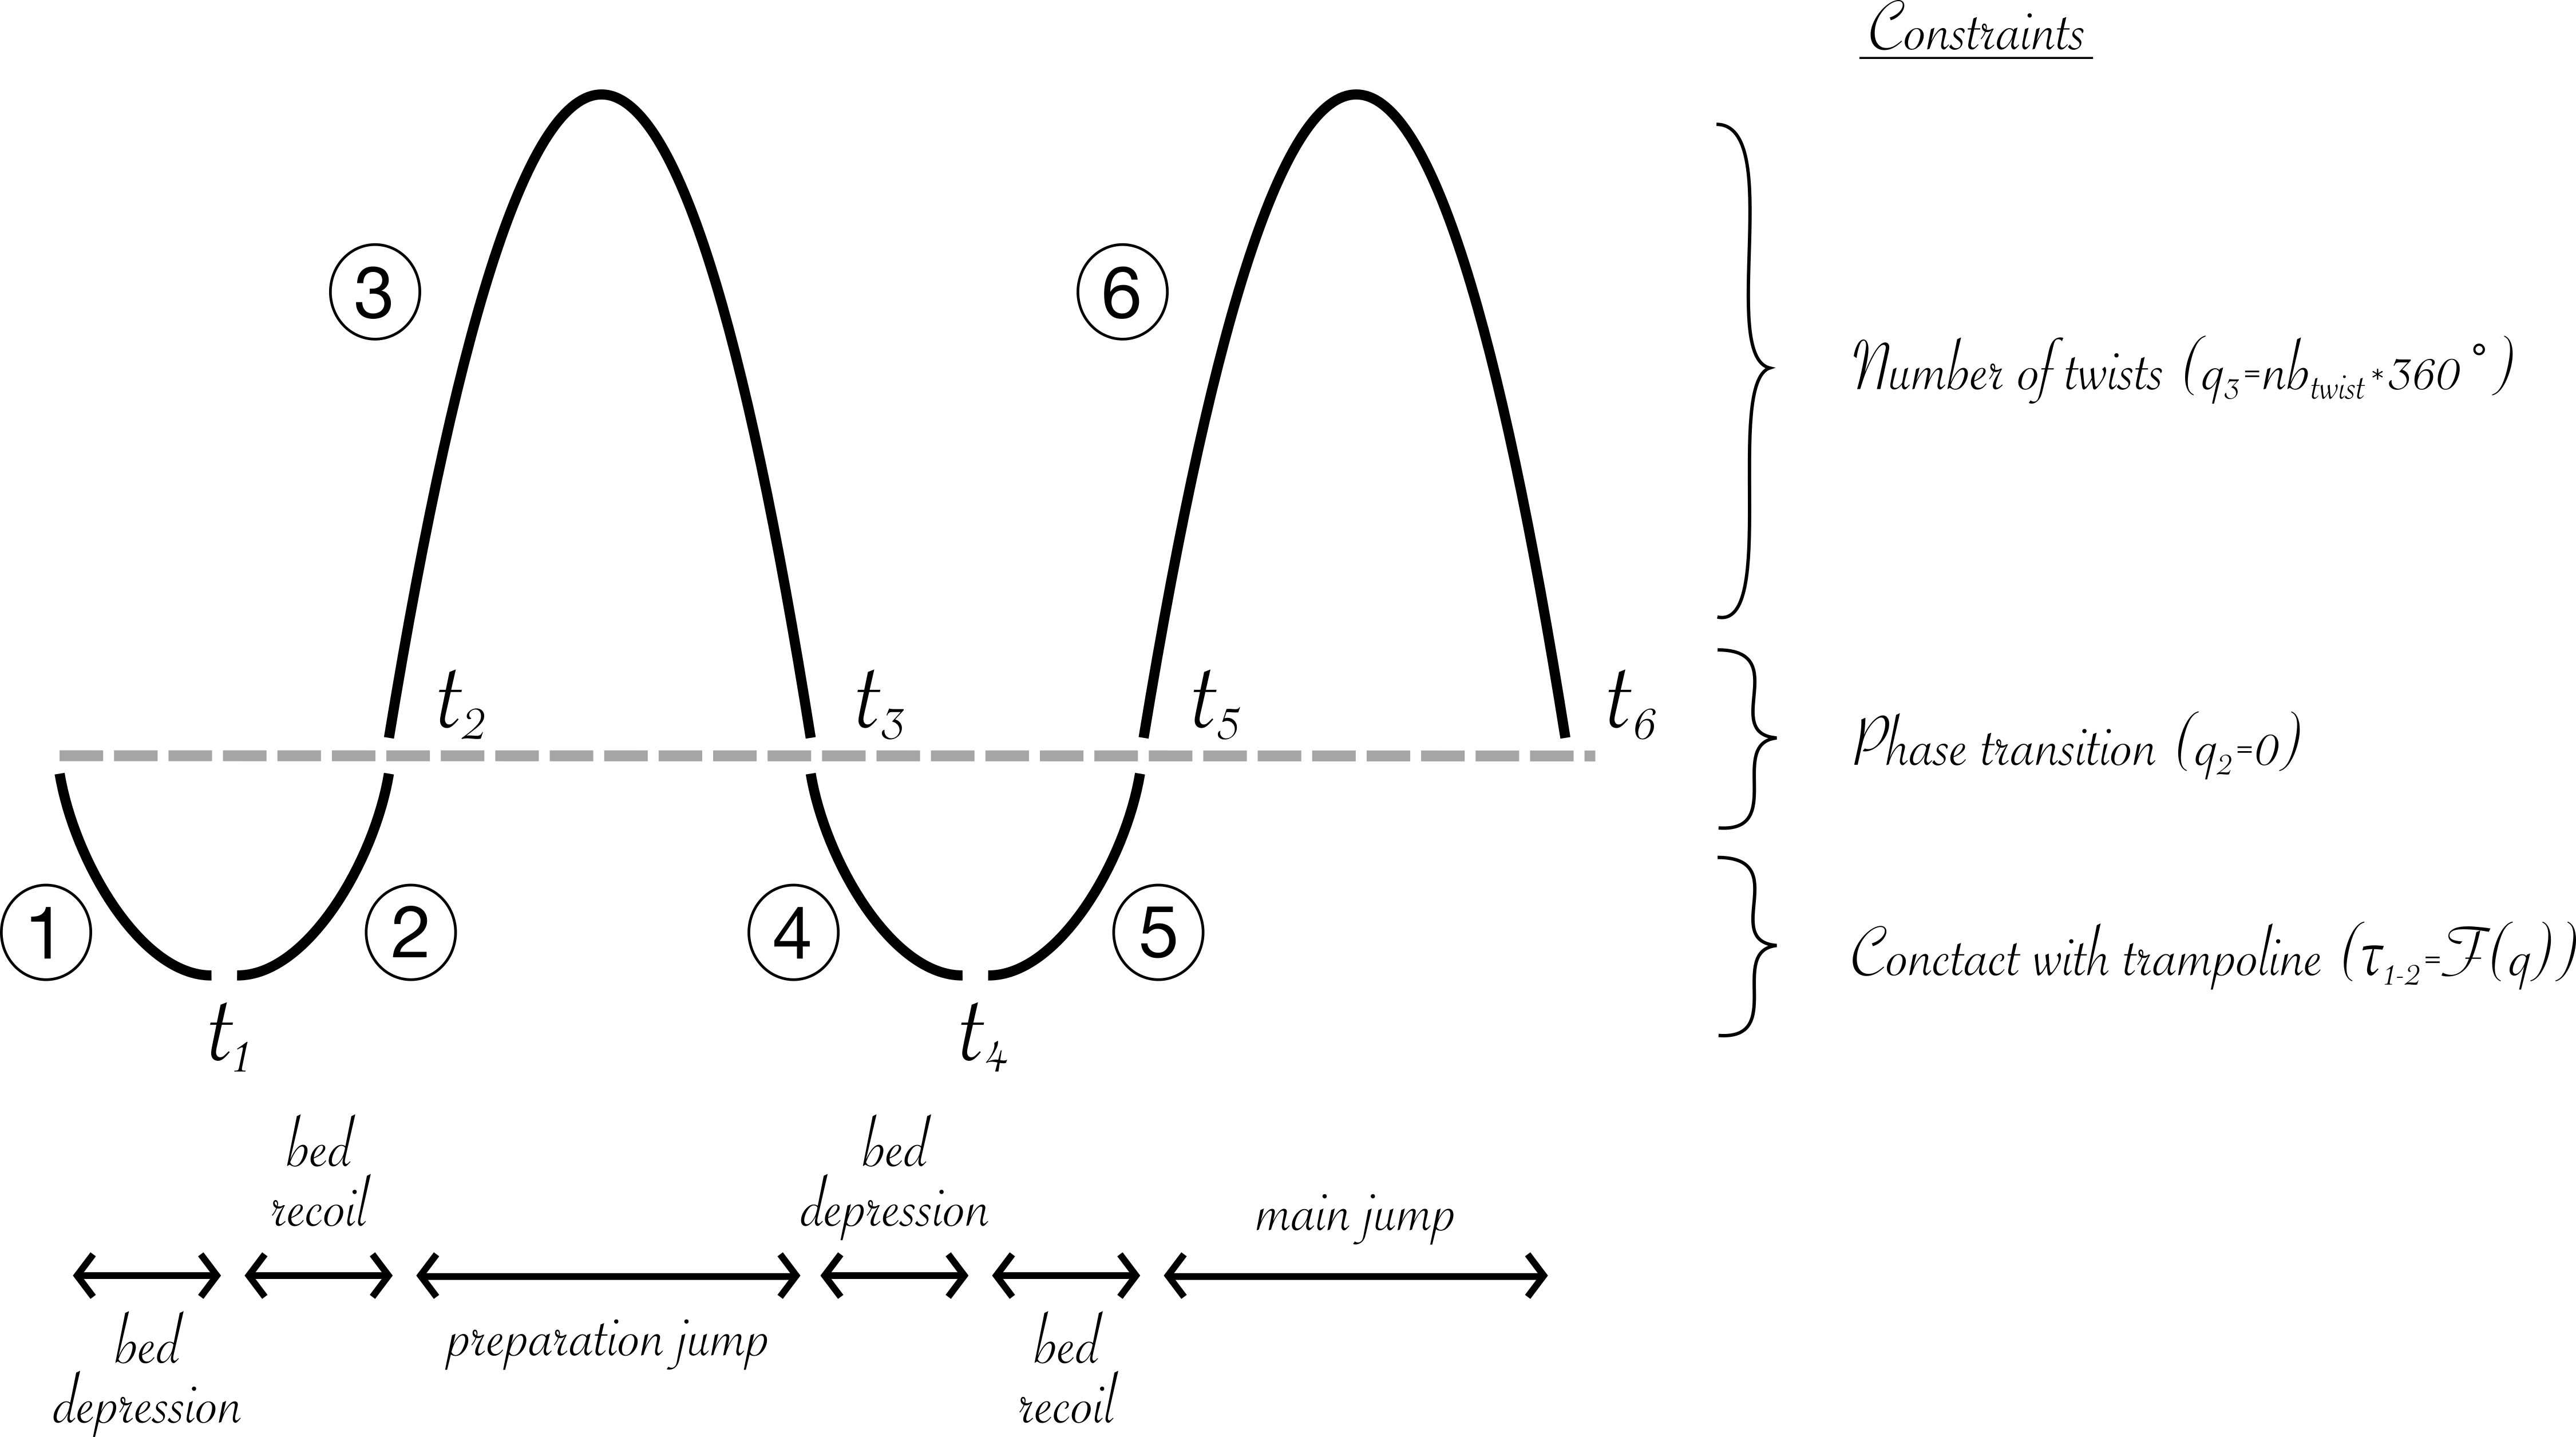
\includegraphics[width=0.5\linewidth]{figures/Model_phases.png}
% \caption{Illustaration of the separation of the OCP in 6 phases.}
% \label{fig:Model_phases}
% \end{figure}


\subsection{Multi-start approach}\label{subsec:2f}
\comEC{départs avant, arrière, avant-arriere, arriere-avant (0, 1, 2, 3, 4, 5 saltos groupé, carpé, tendu) changer la force du modèle}
A multi-start approach was used to explore a wider variety of local optimum \cite{huchez2015local}.
Each OCP (F, B, FB, BF with somersault ranging from 1 to 4) was solved with 50 ??? random initial conditions.
The solution presenting the greatest height for each OCP was saved for later analysis.


\subsection{Biomechanical analysis of the solutions}\label{subsec:2g}
Angular momentum + max CoM height
Deformation history
Faire en sorte que ls force soit appliquée loin du CoM







\section{Results}\label{sec:results}
Gaphs : 
1) Trampoline bed deformation obtained from optimisation (Fig showing mass-points position and springs between them).
2) Optimal solutions (kinogramme bioviz)... description.
3) 
\begin{figure}[h!]
\centering
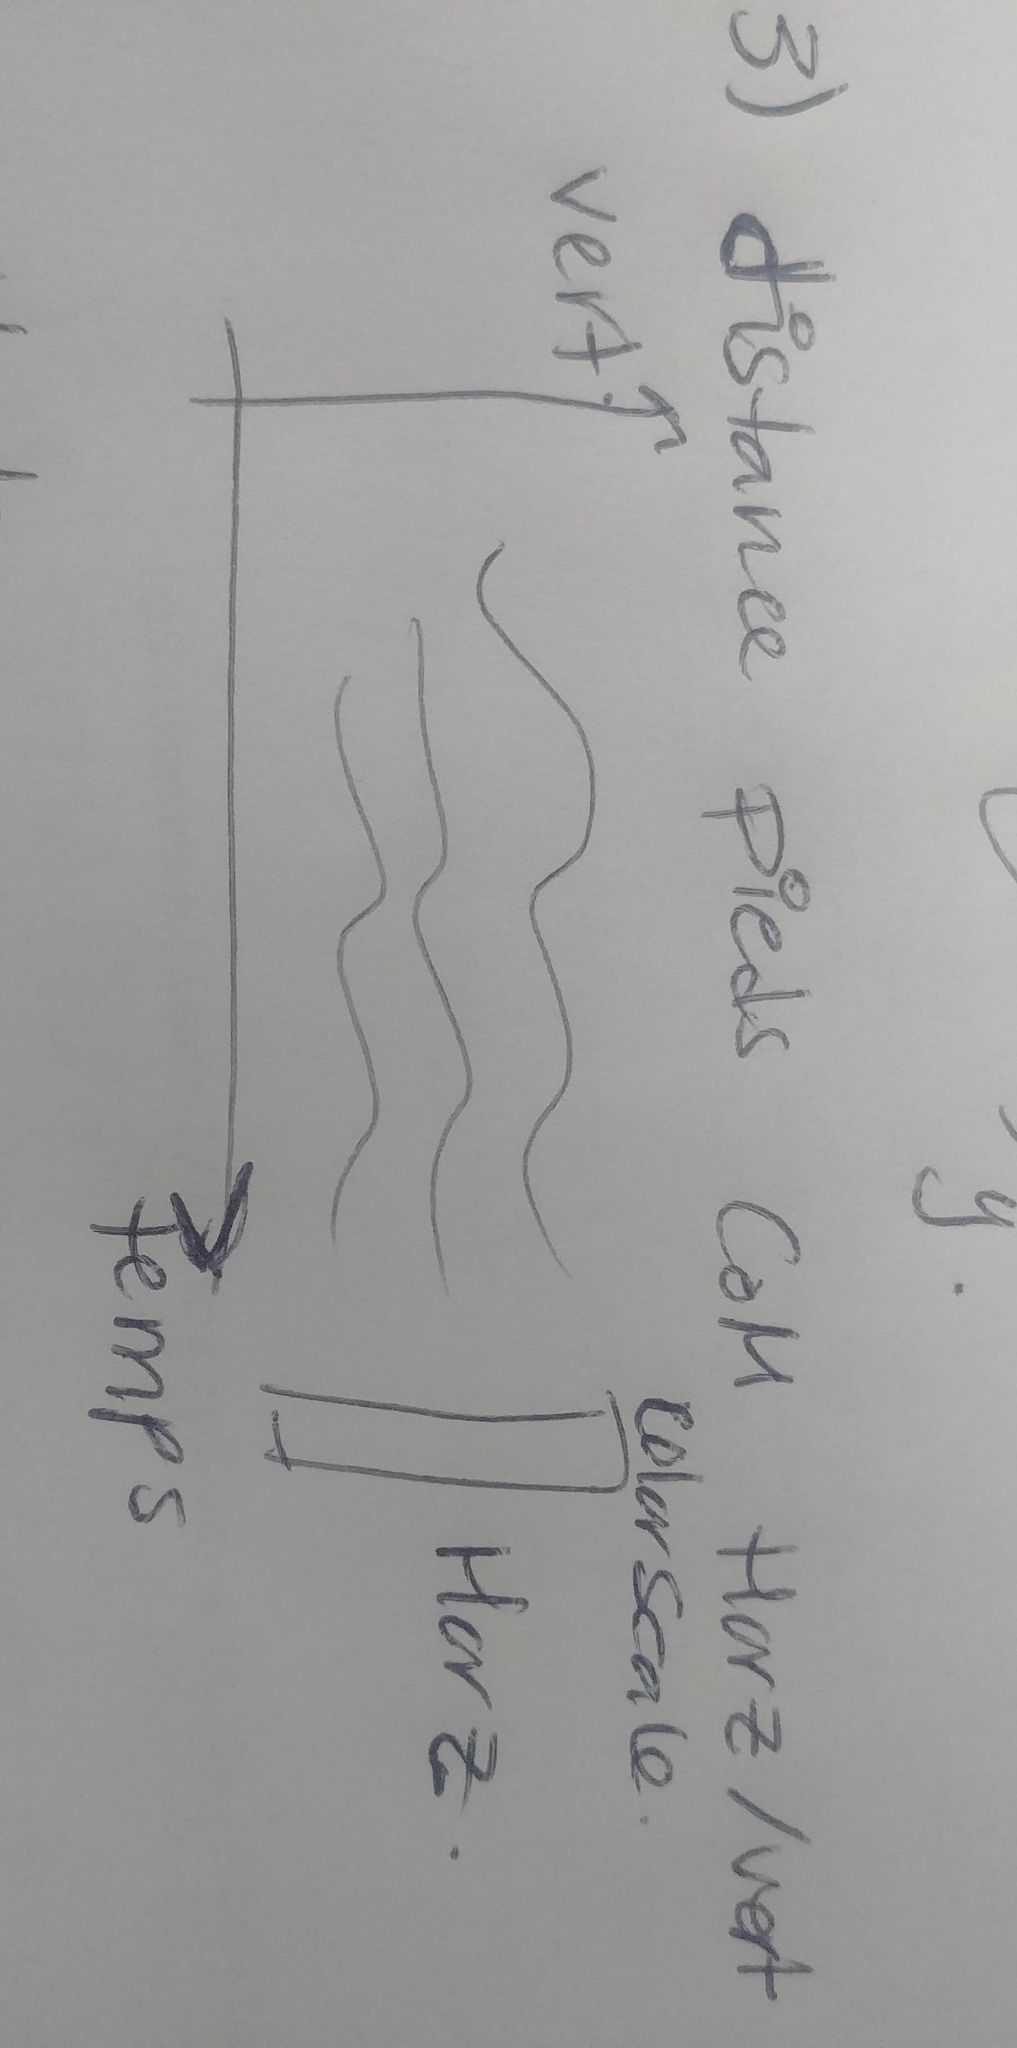
\includegraphics[width=0.5\linewidth, angle =90]{figures/ALaMain_1.jpg}
\end{figure}
4) 
\begin{figure}[h!]
\centering
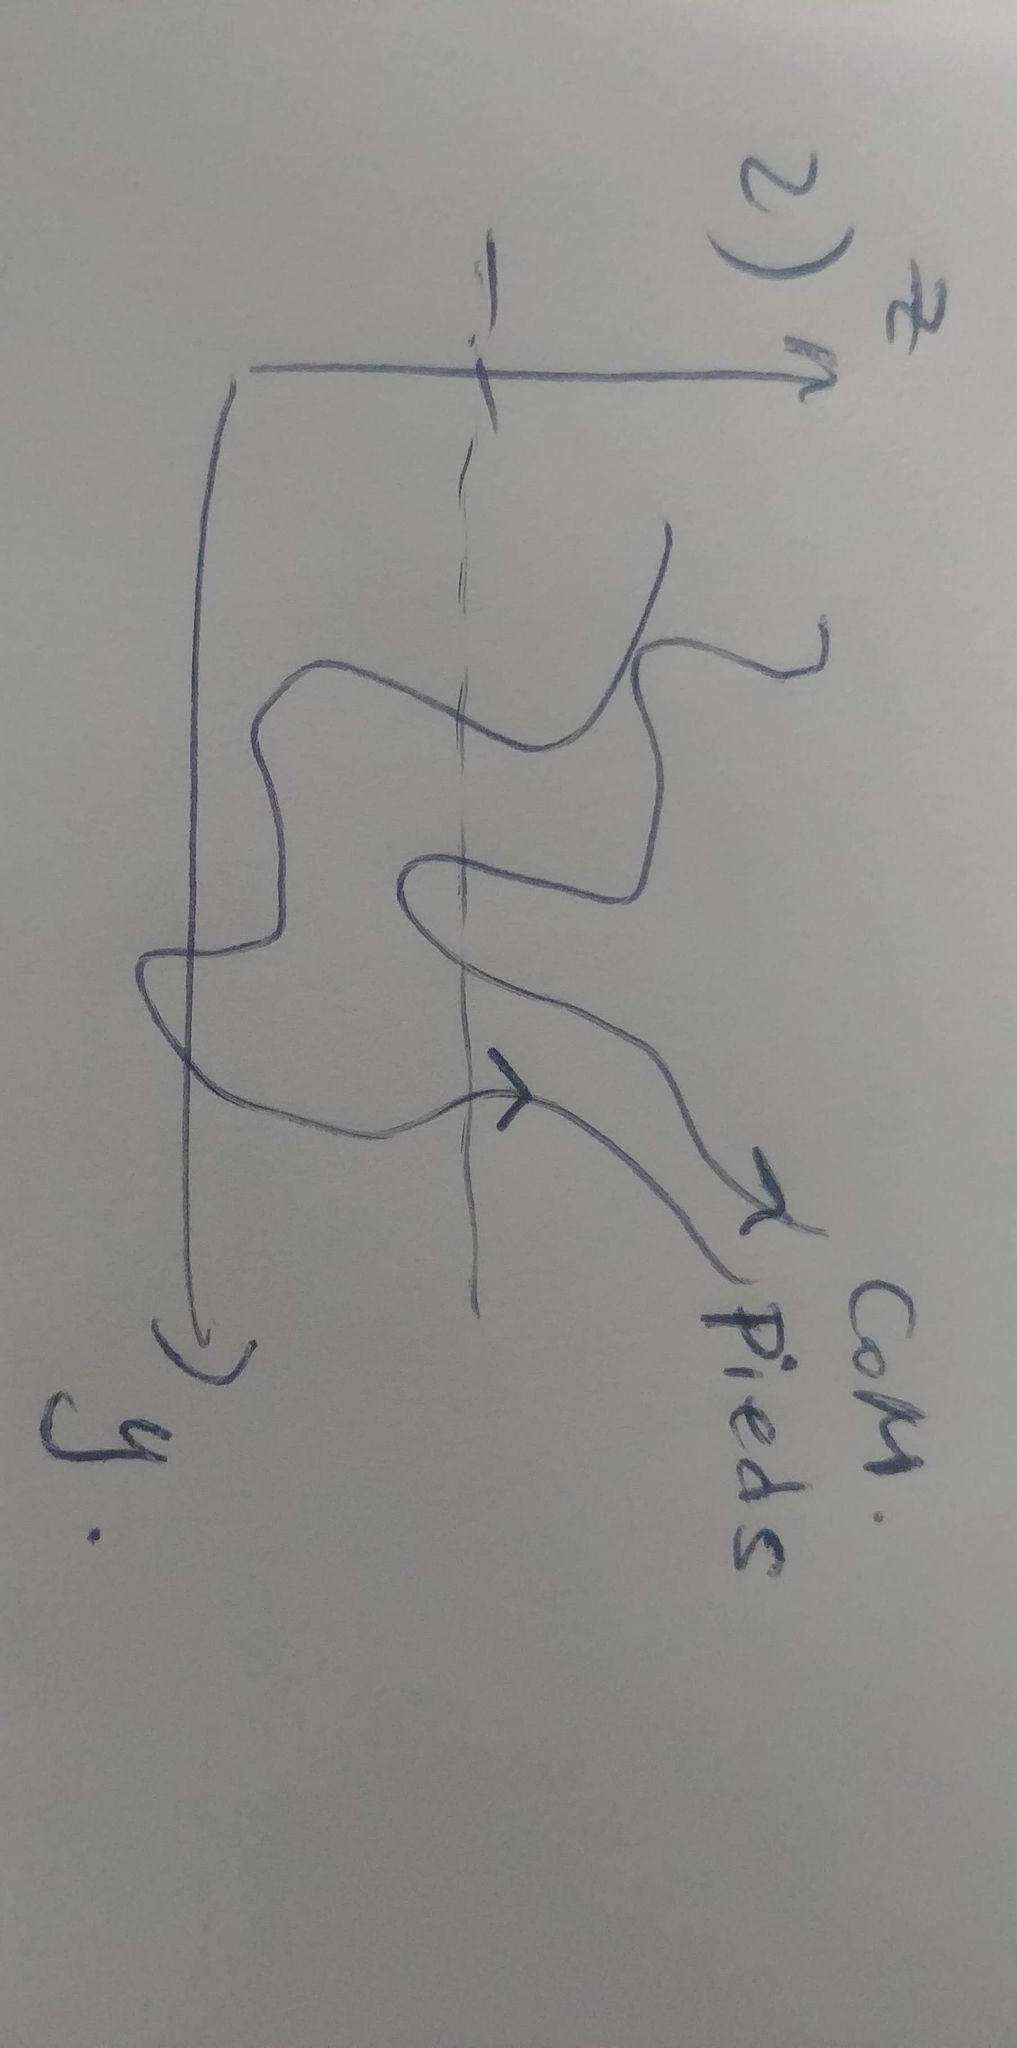
\includegraphics[width=0.5\linewidth, angle =90]{figures/ALaMain_2.jpg}
\end{figure}
5) 
\begin{figure}[h!]
\centering
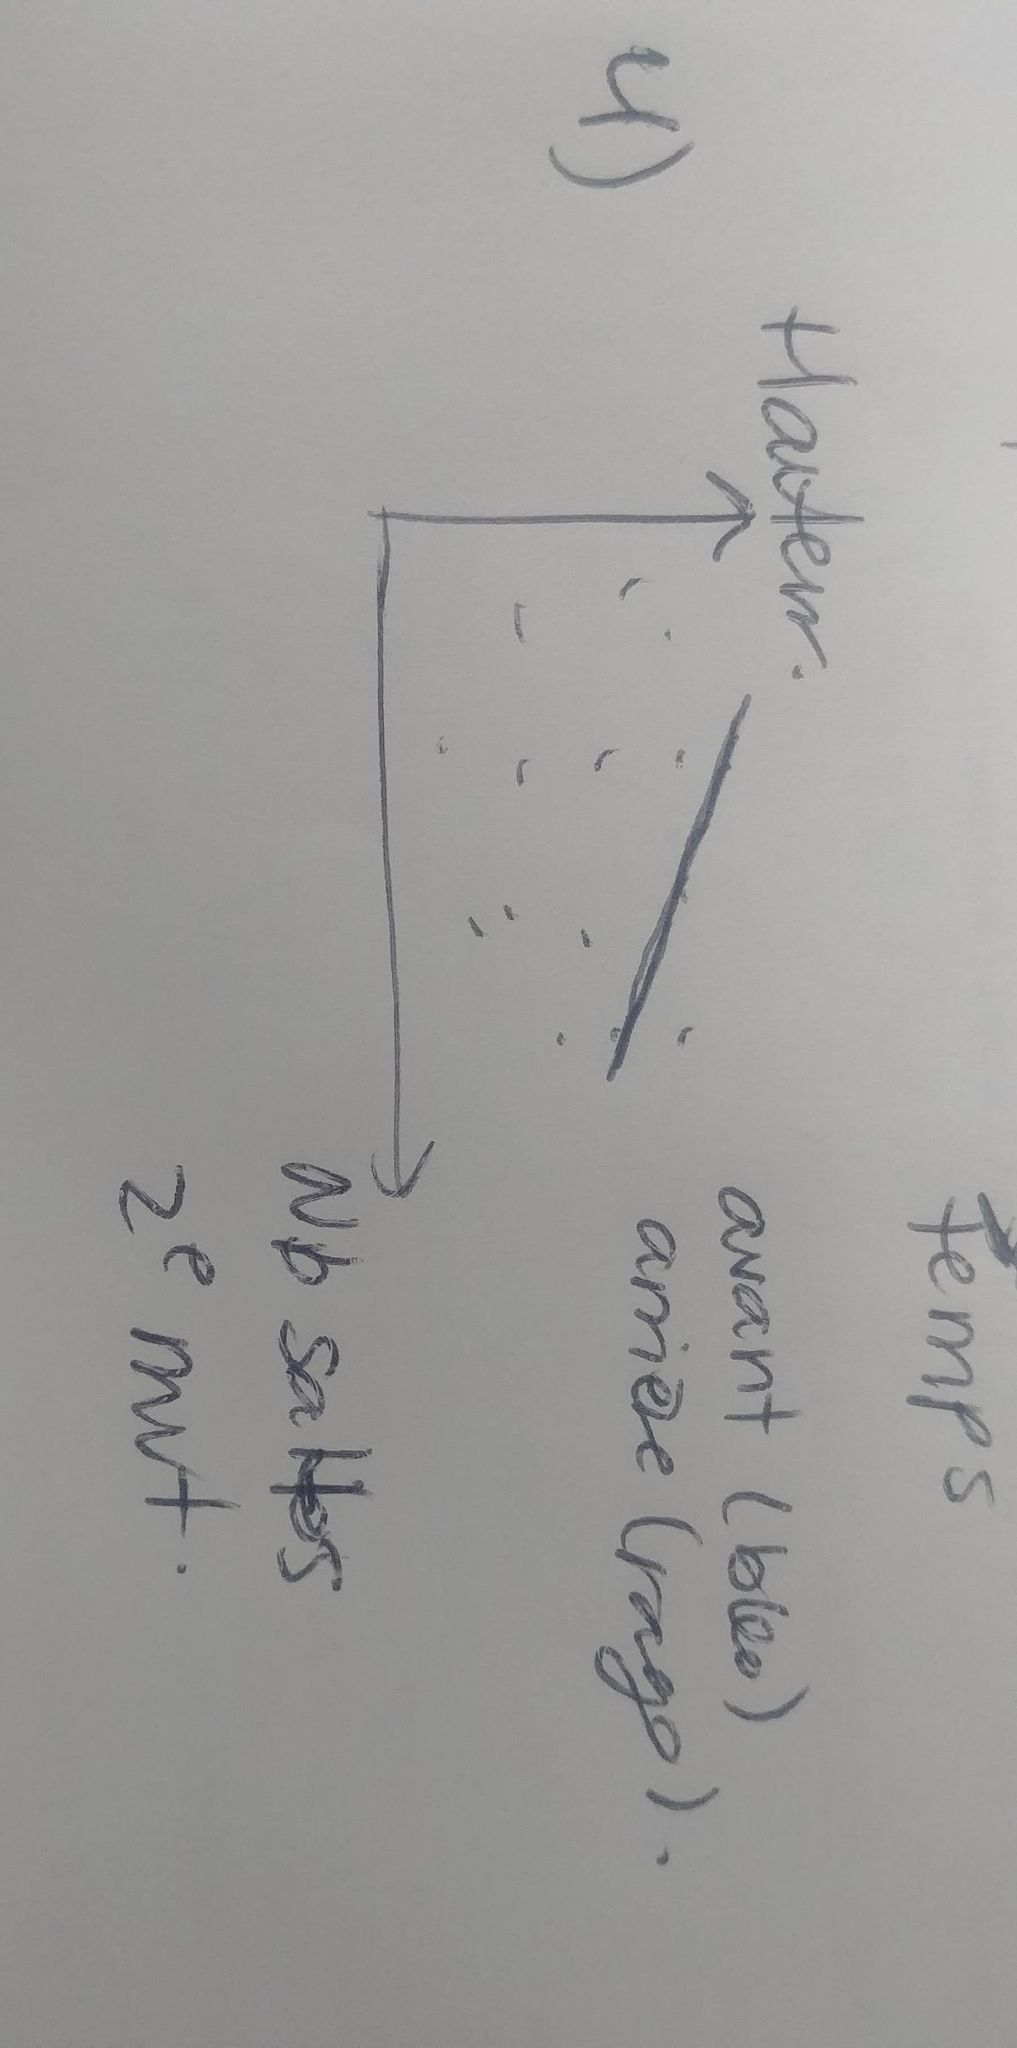
\includegraphics[width=0.5\linewidth, angle =90]{figures/ALaMain_3.jpg}
\end{figure}
6) bras de levier au cours du temps (déplacement toile horz 1 grandeur de la force au cours du contact)
7) Travail vertical et horz en fct du nb de saltos


Aussi
convergence rate.
Est-ce que les torques hit les bounds.



\section{Discussion}\label{sec:discussion}
% The main objective of this study was to generate and analyze innovative and robust twisting techniques to highlight arm strategies that trampolinists could integrate into their practice.
% The main findings are that \textit{(i)} aerial twist performance is linearly correlated to the complexity of arm trajectories, \textit{(ii)} moving the arms in the so-called ``\textit{best tilting plane}'' is an efficient strategy to generate twist rotation and \textit{(iii)} for similar twist performance, 3D techniques are simpler and require less efforts than 2D techniques. 

1) position du CoM au cours du contact \cite{lephartatiner}
2) translation horizontale du a la force verticale (!?!?)
3) positionnement en quittant la toile


\subsection{To be determined}\label{subsec:4a}
To Do


\subsection{Limitations}\label{subsec:4e}
The trampoline used in \cite{} to determine the constants of the model is a 6mm x 4mm is a model of trampoline that is not used any more in FIG competitions.
No damping coefficients (due to air friction through the trampoline web).
Point contact between the feet and the trampoline. (No ankle, no region of depression of the bed)
During the contact phases, the feet are considered attached to the trampoline (No friction coeff has been used to model contact).

\section{Conclusion}\label{sec:conclusion}
% This research shows that athletes could gain in performance by incorporating 3D motions to their techniques, especially by moving their segments in the best tilting plane (i.e., plane formed by the twist and angular momentum axes).
% We provided three innovative and simple 3D arm techniques for a triple twist backward somersault robust to kinematic perturbations. 
% The selected 3D arm techniques were less complex, required less efforts and had better potential for landing than the equivalent 2D technique, establishing the superiority of 3D arm techniques.
% With the comprehension brought by this work, coaches could better guide their future athletes throughout the learning of 3D arm techniques.


\setcitestyle{number}
\bibliographystyle{elsarticle-num} 
\bibliography{biblio}

\clearpage

\begingroup
\let\clearpage\relax 
\onecolumn 
\section{Appendix}\label{sec:appendix}
\subsection{To be determined.}\label{subsec:5a}
To Do

\endgroup




\end{document}
